\section{A Javadoc Extension for Public Contracts}
\label{sec:approach}

%update to be more general
To perform studies on public contract styles, we propose \contractjdoc{}, a simple extension to the Javadoc-tagging systems with contracts. Its compilation system is built on the top of the AspectJML compiler~\cite{aspectjml}, providing support for runtime checking of the contracts.
\contractjdoc{} allows programmers to document \emph{contract expressions} amid Javadoc header for methods. With just a few new tags, in addition to the standard Javadoc tags, one can write contracts as Javadoc comments that are compiled to runtime checkable code. 
%The \contractjdoc{} approach fulfills the gap between informal documentation (as with Javadoc) and formal specification (such as JML~\cite{jml} or Code Contracts~\cite{codeContractsPaper}).

In the remaining of this section, we present, based on a running example, how \contractjdoc{} supports a mixed approach, which combines textual documentation with a limited set of formal features from the examples in Section~\ref{sec:example}.

\subsection{Language Extension Design}

The \contractjdoc{} tags act as traditional Javadoc tags,  embedded within block comments. 
The main idea is to allow a mix between the traditional Javadoc syntax and JML-like notation; 
JML seems appropriate in this context since it is built over Java expressions, except for a few logical operators (such as \texttt{==>} -- implication).
Embedding contracts allows for contract expressions (e.g., pre-conditions) in the existing Javadoc comments
and making them machine discoverable through the use of
marker brackets within those comments.
%semantic-neutral
In this proposal, we consider the textual comments surrounding the formal expressions semantically neutral -- we assume the expression does not change its semantics. 

%benefits
The potential benefit of embedding contract expressions in a more natural setting for the developer is his/her ability to remain within a single artefact which is purpose-built for writing public specifications. 
This is especially true because the overwhelming majority of contracts that programmers write in
practice are short and simple~\cite{Estler-etal14,typeContracts}. For instance, in 75\% of Code Contracts~\cite{codeContractsPaper} projects, the written contracts are basic checks for the presence of data (e.g., non-null checks)~\cite{typeContracts}. In such scenarios, there is no additional effort in embedding such contracts in Javadoc comments using our \contractjdoc{} approach.

\subsubsection{Pre-conditions}
%Recall the pre-condition illustrated in Section~\ref{sec:example}. We discussed two ways to document such a pre-condition, a formal one in JML (see Figure~\ref{Fig-JML-Bank}) and an informal one with plain Javadoc comments (see Figure~\ref{Fig-Javadoc-Bank}).
In \contractjdoc, the pre-condition for method \lstinline!withdraw! from Section~\ref{sec:example} can be rewritten as the excerpt in Figure~\ref{fig:pre-example}.

\begin{figure}
\centering
\begin{lstlisting}[basicstyle=\footnotesize\ttfamily,name=figxpi, frame=lines, mathescape=true]
 /**
  * @param amt the amount value to withdraw, 
  *   where $\shd{[amt > 0 \&\& amt <= balance]}$
  */
 double withdraw(double amt) 
   throws TransactionException {...}
\end{lstlisting}
\caption{\texttt{withdraw}'s pre-condition.}
\label{fig:pre-example}
\end{figure}

%explain
Tag \lstinline!@param! documents parameter \lstinline!amt! of \lstinline!double! type.
Besides the usual comments, we have added a boolean expression
surrounded by brackets; these brackets indicate assertions internally to the \contractjdoc{} compiler, so the comments can be turned into an executable pre-condition checking.
An alternative (not showed) is to replace tag \lstinline!@param! by \lstinline!@requires! or \lstinline!@pre!. Both can be used to document a pre-condition constraint; the main difference is that they are not part of the standard Javadoc tagging system.

\subsubsection{Post-conditions}

We may use \contractjdoc{} for post-conditions as the example in Figure~\ref{fig:post-example}.


\begin{figure}
\centering
\begin{lstlisting}[basicstyle=\footnotesize\ttfamily,name=figxpi, frame=lines, mathescape=true]
 /**
  * @return amt the current balance after withdraw,
  *   that is $\shd{[@return == balance]}$
  * @throws TransactionException the 'balance' does
  *  not change, that is $\shd{[balance == @old(balance)]}$
  */
 double withdraw(double amt) 
   throws TransactionException {...}
\end{lstlisting}
\caption{\texttt{withdraw}'s post-condition.}
\label{fig:post-example}
\end{figure}

Tags \lstinline!@return! and \lstinline!@throws! document normal and exceptional post-conditions, respectively, with their respective expressions
expressed within brackets.
%Tag \lstinline!@return! appears again within the brackets. This inner is allowed (in \contractjdoc{}) and allows one
%to use the value of the method's returns to write the contract regarding
%the normal post-condition. A similar tag, \lstinline!@result! derived from the JML syntax,
%can also be employed instead of the inner use of the \lstinline!@return! tag.
Tag \lstinline!@old! refers to expressions or fields in their pre-state, used only in post-conditions.

As with pre-conditions, \contractjdoc{} offers three tags for expressing post-conditions.
For normal post-conditions, similar JML-based tags \lstinline!@ensures! and \lstinline!@post! may be used instead of \lstinline!@return!.
For \lstinline!@throws! tag, the standard Javadoc offers a surrogate tag \lstinline!@exception!. 
Derived from JML, we can also employ \lstinline!@signals! to document and constrain exceptional behaviour.

% \subsubsection{Documenting Invariants}

% Beyond the support for pre- and post-conditions, \contractjdoc{} make the use of invariants also
% available by means of \texttt{@inv} tags.
% The format of writing is the same as those
% for pre- and post-conditions.
% The difference is related to the semantics: while pre- and post-conditions apply to a specific
% method, an invariant applies for all methods from a class. For invariants, we follow the
% semantics of the JML language. For more information, please refer
% to~\cite{jml}.
% The invariant contract, described in Section~\ref{sec:example}, can be written
% as follows:
% \begin{lstlisting}[basicstyle=\footnotesize\ttfamily,name=figxpi, frame=lines, mathescape=true]
% class BankAccount {
%  /**
%   * @inv The overall balance should be $\shd{[balance >= 0]}$
%   */
%  double balance;
%  //...
% }
% \end{lstlisting}
% Invariant declarations may be placed above the field
% declarations (as in the example), or  above the
% class declaration as a valid Javadoc block comment.

\subsection{Supporting Infrastructure}

The \contractjdoc{} compiler is based on the open source AspectJML/ajmlc compiler~\cite{aspectjml,ajmlc,Rebelo-etal08}.
Unlike the standard JML compiler jmlc~\cite{jmlc-compiler}, ajmlc presents code optimisations and improved error reporting~\cite{ajmlc}.
Also, AspectJML enables the modularisation
of crosscutting contracts that can arise in standard
JML specifications~\cite{aspectjml}.

We adapted the front-end of the AspectJML/ajmlc compiler to convert/preprocess the \contractjdoc{} tags into the corresponding JML features, like pre- and post-conditions.
After conversion, the compilation occurs as usual and generates aspects to runtime checking the
contracts. See Figure~\ref{fig:compilerInfra}
for an overview of the compilation strategy.
First, source code with \contractjdoc{}
contract expressions goes through a tag processor and a type checker. Next, a runtime assertion aspect is generated, which is woven to the source code by the Aspectj compiler, producing bytecode with assertions, amenable to runtime checking.


\begin{figure}[h]
\centering
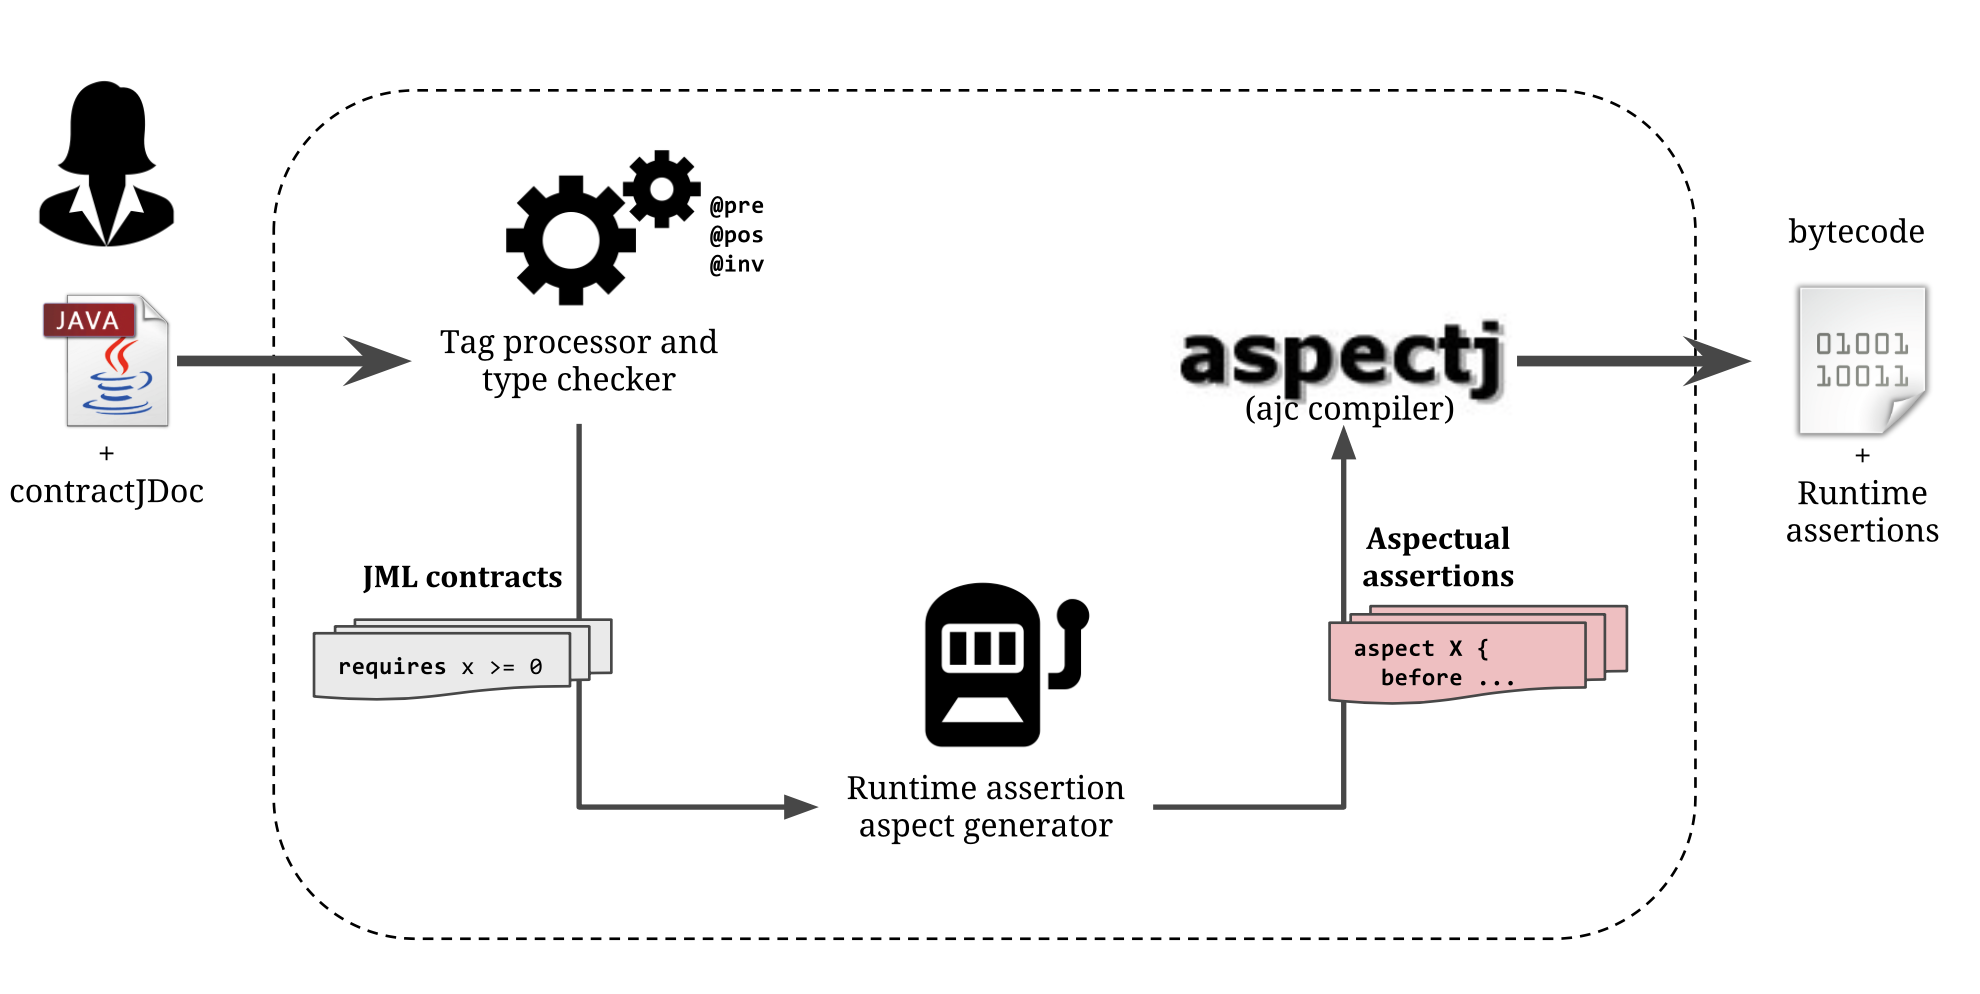
\includegraphics[width=1.0\textwidth]{figs/compilerInfra}
\caption{Compilation Infrastructure for ContractjDoc.}
\label{fig:compilerInfra}
\end{figure}

